\section{Strengths and weaknesses}
	Summarizing, this document shows a vision-based tracking algorithm to be used by UAVs. This algorithm is able to target multiple objects based on their color. This last sentence is the main advantage if it's compared with other algorithms as CAMSHIFT's \cite{blablacam} and so on. The bottle neck of color-based algorithm use to be the computational time, however, our implementation allows to UAV to process fastly the taken pictures. In both cases the algorithm processes faster than 40 pictures by second.
	The algorithm was tested on many simulations inside the V-REP application and using a variety of datasets provided by the GRVC. In both cases, estimation's error is less than a 10\% of the distance between the target and the camera.
	In parallel of the developing of the algorithm, we develop a library in order to make it easy to use, not only inside this project, but in many applications. Chapter 7 \ref{chap:c7_annex} have a brief description of this library.
	
	% % TODO 666 ADD CITES!!
	
\section{Future Branches}
	BLA BLA BLA INTRO BLA BLA BLA
	In this section we propose some possible improvements for the algorithms or the application's architecture.
	
	\subsection{Parallel Color Clustering}
	One of the bottle necks of the algorithm is the color clustering or color segmentation of the image. Every step of the algorithm requires to check every single pixel of the input images. This fragment of the process is easily implementable under the parallel paradigm.
	GPU's cores are slower than general CPU's cores. However there are more cores in GPU than in CPU \ref{fig:gpu}, so parallelization in GPU can highly improve the global speed of the process.
	
	% % TODO 666 ADD CITES!!
		
	\begin{figure}[ph]
		\centering
		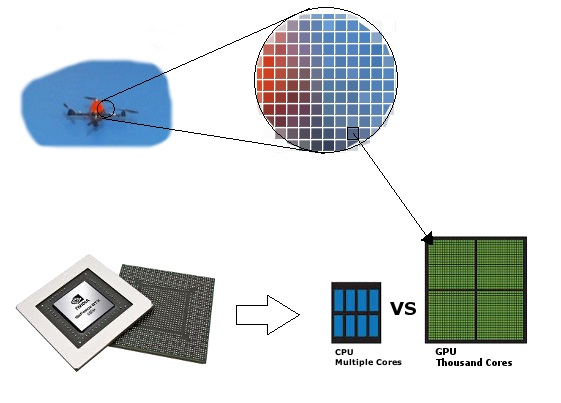
\includegraphics[width=0.7\linewidth]{../Images/c5/gpu}
		\caption{Parallelization}
		\label{fig:gpu}
	\end{figure}


	\subsection{Shape recognition}
	At present, the criteria of choosing the target is by size and color. Nevertheless, where there are multiple possible targets in the scene it could confuse them or divide them if they are composed of more than one color. So shape recognition should be an useful tool to differentiate many objects once they were segmented.
	
	% % TODO Add image of shape segmentation
	
	% % TODO 666 ADD CITES!!
		
	\subsection{Higher Conscience}
	Finally another improvement (this one about the complete architecture of the software) is the addition of a higher conscience or AI that could arrange the amount of information and use it to improve the tracking.
	For example, storing the information about the geometrical position and speed of the targets associated with their shape and color the algorithm will be able to estimate separately their behavior.
	
	
	% % TODO Add image of shape segmentation
		
	% % TODO 666 ADD CITES!!
		
